\documentclass[twoside]{article}
\usepackage[a4paper]{geometry}
\geometry{verbose,tmargin=2.5cm,bmargin=2cm,lmargin=2cm,rmargin=2cm}
\usepackage{fancyhdr}
\pagestyle{fancy}

% nastavení pisma a~češtiny
\usepackage{lmodern}
\usepackage[T1]{fontenc}
\usepackage[utf8]{inputenc}
\usepackage[czech]{babel}

% odkazy
\usepackage{url}

\usepackage{float}
% vícesloupcové tabulky
\usepackage{multirow}
\usepackage{amssymb}
\usepackage{gensymb}
\usepackage{bbold}
\usepackage{mathtools}
\usepackage{commath}

% vnořené popisky obrázků
\usepackage{subcaption}

% automatická konverze EPS 
\usepackage{graphicx} 
\usepackage{epstopdf}
\usepackage{amsmath}
\epstopdfsetup{update}

% odkazy a~záložky
\usepackage[unicode=true, bookmarks=true,bookmarksnumbered=true,
bookmarksopen=false, breaklinks=false,pdfborder={0 0 0},
pdfpagemode=UseNone,backref=false,colorlinks=true] {hyperref}

% Poznámky při překladu
\usepackage{xkeyval}	% Inline todonotes
\usepackage[textsize = footnotesize]{todonotes}
\presetkeys{todonotes}{inline}{}
\graphicspath{{./images}}

%https://tex.stackexchange.com/questions/2783/bold-calligraphic-typeface
\DeclareMathAlphabet\mathbfcal{OMS}{cmsy}{b}{n}

% Zacni sekci slovem ukol
\renewcommand{\thesection}{Úkol \arabic{section}}
% enumerate zacina s pismenem
\renewcommand{\theenumi}{\alph{enumi}}

% smaz aktualni page layout
\fancyhf{}
% zahlavi
\usepackage{titling}
\fancyhf[HC]{\thetitle}
\fancyhf[HLE,HRO]{\theauthor}
\fancyhf[HRE,HLO]{9. prosince 2021}
 %zapati
\fancyhf[FLE,FRO]{\thepage}

% údaje o autorovi
\title{Robotika - Kalibrace paralelního manipulátoru}
\author{Vojtěch Michal}
\date{9. prosince 2021}

\begin{document}

\maketitle

\section{Kalibrační body}
Pro maximálně rovnoměrnou kalibraci ve všech rozumných bodech pracovního prostoru byly kloubové souřadnice vybírány z kartézského součinu
množin
\begin{equation}
	\begin{split}
		\Theta = \left\{0, \pm \frac{\pi}{6}, \pm \frac{\pi}{4}, \pm \frac{\pi}{3}, \pm \frac{\pi}{2}, \pm \frac{2\pi}{3}, \pm \frac{3\pi}{4},\pm \frac{5\pi}{6}, \pi \right\},  \\
		D = \left\{1,3,5,7,9,11,13,15,17,19,21\right\}.
	\end{split}
\end{equation}
To dohromady činí $\vert\Theta\vert \cdot \vert D \vert = 16 \cdot 11 = 176$ bodů tvaru
\begin{equation}
	\begin{bmatrix}
		d_1 \\ \theta_2
	\end{bmatrix} \text{, kde } d_1 \in D \text{ a } \theta_2 \in \Theta.
\end{equation}

\section{Konvergence numerické metody}

V grafech \ref{fig:chyba} jsou vyneseny průběhy akumulované globální chyby v závislosti na indexu iterace numerického optimalizačního algoritmu
pro dva různé experimety. Graf \ref{fig:chyba_log} pro snazší čitelnost využívá logaritmické svislé osy.
Rychlost konvergence pro různé experimenty není rovnoměrná, i ve velmi pomalém příkladě (jako je \ref{fig:chyba_lin}) již první čtyři 
iterace stačí k zatlačení normy chybového vektoru pod hodnotu 1.
Na konci algoritmu je chyba v řádu $10^{-4}$ dm, tedy 0.01 mm, a méně.

\begin{figure}[htbp]
	\centering
	\begin{subfigure}{0.45\linewidth}
		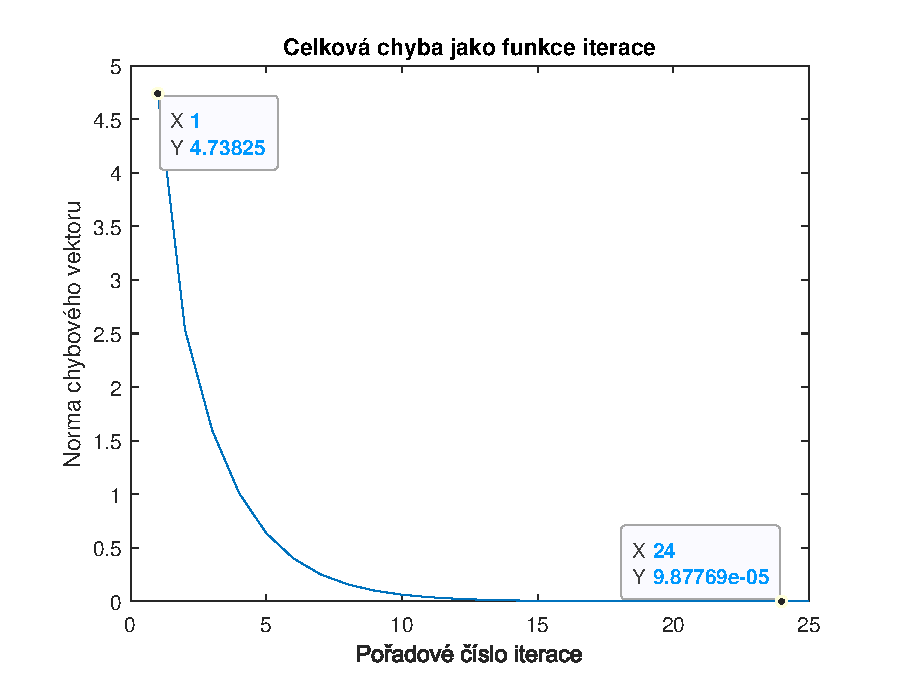
\includegraphics[width=\linewidth]{chyba.eps}
		\caption{Lineární osy x, y}
		\label{fig:chyba_lin}
	\end{subfigure}
	\begin{subfigure}{0.45\linewidth}
		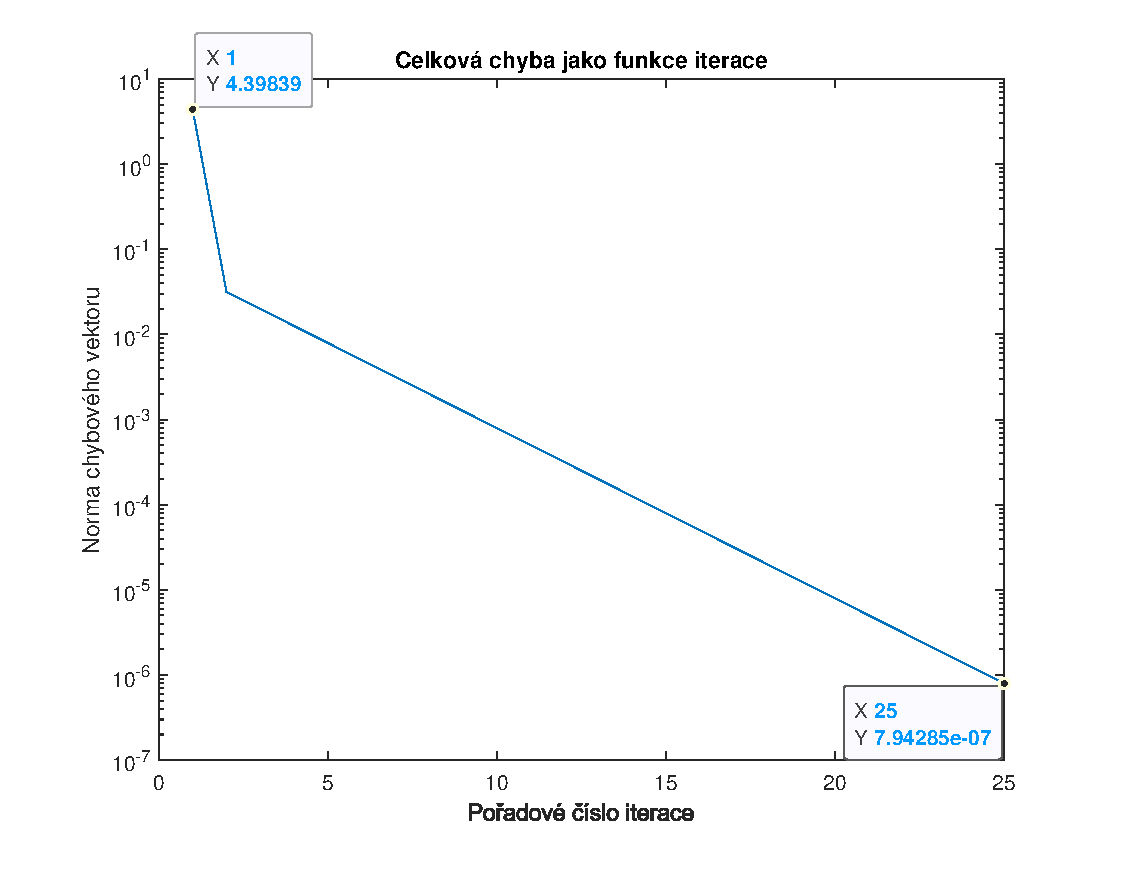
\includegraphics[width=\linewidth]{chyba_semilog.eps}
		\caption{Lineární osa x, logaritmická osa y}
		\label{fig:chyba_log}
	\end{subfigure}
	\caption{Závislost zbytkové globálníchyby na iteraci kalibračního algoritmu}
	\label{fig:chyba}			
\end{figure}

\section{Nákres}

Na obárzku \ref{fig:nakres} jsou rukou psané poznámky k úloze a náčrtek s významem jednotlivých proměnných.

\begin{figure}[htbp]
	\centering
	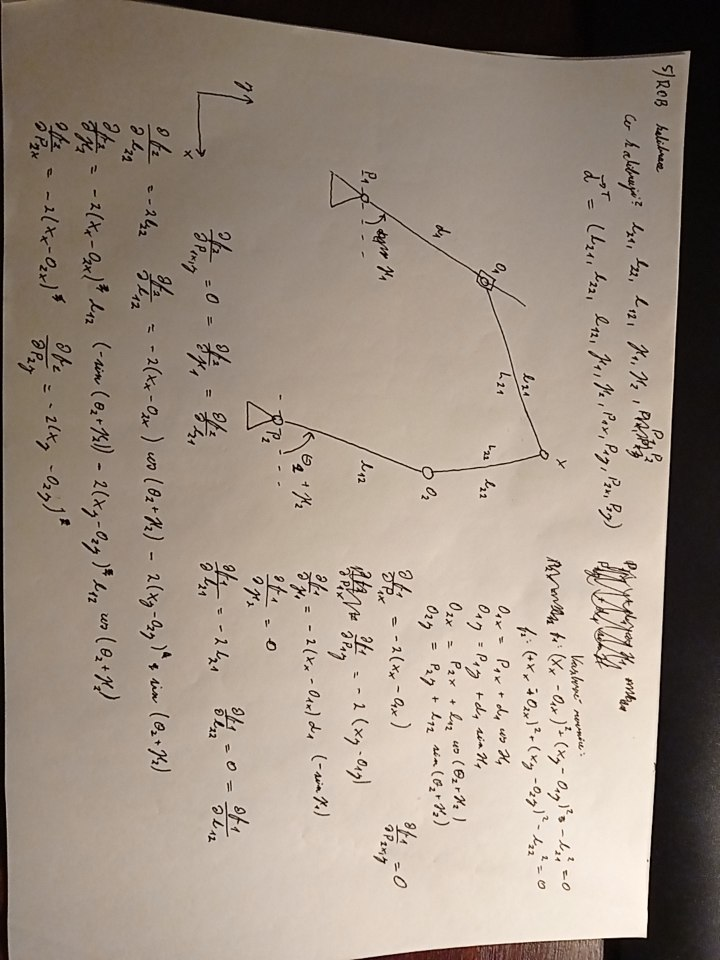
\includegraphics[width=\linewidth]{nakres.jpg}
	\caption{Nákres úlohy a ručně psané poznámky}
	\label{fig:nakres}	
\end{figure}

\end{document}


